\documentclass[tikz,border=10pt]{standalone}
\usepackage{tkz-euclide} % 基于TikZ，专门用于平面几何绘图

\begin{document}
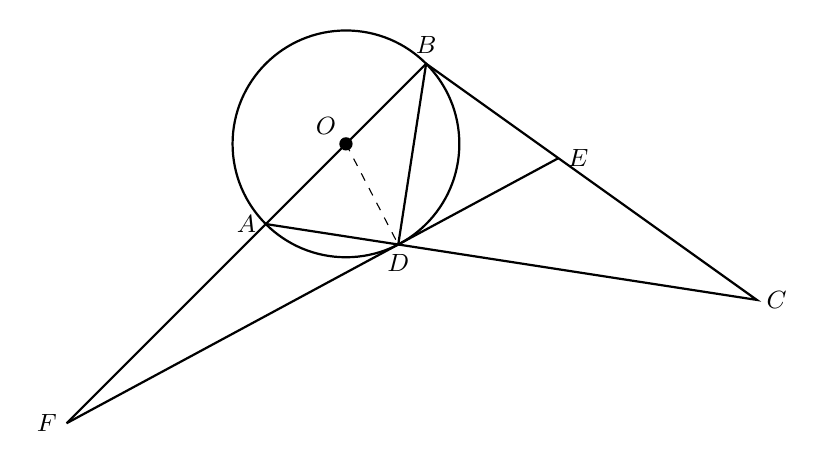
\begin{tikzpicture}[scale=1.2, font=\small]
    % 1. 定义圆心 O 和半径
    \coordinate (O) at (0,0);
    \def\radius{1.2}

    % 2. 定义直径端点 A 和 B (设为 45 度角斜置以符合原图视感)
    \coordinate (A) at (225:\radius);
    \coordinate (B) at (45:\radius);

    % 3. 绘制圆 O
    \draw[thick] (O) circle (\radius);

    % 4. 计算切线方向并定位 C 点
    % B 是切点，BC 垂直于 OB
    \coordinate (C) at ($(B) + (0:3.5) + (-90:2.5)$); % 根据视觉比例调整负载点

    % 5. 寻找圆上的点 D 并连接 AC
    % 原图中 D 在圆周上，且 A, D, C 三点共线
    \path[name path=circle] (O) circle (\radius);
    \path[name path=lineAC] (A) -- (C);
    \path [name intersections={of=circle and lineAC, by={D_temp, D}}];

    % 6. 定义 E 点 (在 BC 上)
    % 寻找 F 点 (BA 延长线与 ED 延长线的交点)
    % 先根据视觉确定 E 的位置
    \coordinate (E) at ($(B)!0.4!(C)$);

    % 7. 计算 F 点 (直线 BA 与直线 ED 的交点)
    \coordinate (F) at (intersection of B--A and E--D);

    % 8. 绘制直线和线段
    \draw[thick] (F) -- (B) -- (C) -- (A) -- cycle; % 绘制大框架
    \draw[thick] (B) -- (D); % 弦 BD
    \draw[thick] (F) -- (D) -- (E); % 线段 FD 和 DE

    \draw[dashed] (O) -- (D);

    % 9. 标注点和符号
    \fill (O) circle (1.5pt) node[above left] {$O$};
    \node[left] at (A) {$A$};
    \node[above] at (B) {$B$};
    \node[right] at (C) {$C$};
    \node[below] at (D) {$D$};
    \node[right] at (E) {$E$};
    \node[left] at (F) {$F$};

    % 10. 细节微调：在 O 点画一个小圆点表示强调
    \fill (O) circle (2pt);

\end{tikzpicture}
\end{document}